\documentclass{book}
\usepackage[utf8]{inputenc}
\usepackage{fullpage}
\usepackage{graphicx}
\usepackage{sansmath}
\usepackage{amsmath}
\usepackage{amssymb}
\usepackage[dutch]{babel}
\usepackage{vub}
\usepackage{hyperref}
\usepackage{float}
\usepackage{listings}
\usepackage{color}
\usepackage{tabularx}

\usepackage{listings}
\usepackage{color}
\usepackage{textcomp}
\definecolor{mygreen}{rgb}{0,0.6,0}
\definecolor{mygray}{rgb}{0.5,0.5,0.5}
\definecolor{mymauve}{rgb}{0.58,0,0.82}

\lstset{ %
  backgroundcolor=\color{white},   % choose the background color; you must add \usepackage{color} or \usepackage{xcolor}
  basicstyle=\footnotesize,        % the size of the fonts that are used for the code
  breakatwhitespace=false,         % sets if automatic breaks should only happen at whitespace
  breaklines=true,                 % sets automatic line breaking
  captionpos=b,                    % sets the caption-position to bottom
  commentstyle=\color{mygreen},    % comment style
  deletekeywords={...},            % if you want to delete keywords from the given language
  escapeinside={\%*}{*)},          % if you want to add LaTeX within your code
  extendedchars=true,              % lets you use non-ASCII characters; for 8-bits encodings only, does not work with UTF-8
  frame=single,                    % adds a frame around the code
  keepspaces=true,                 % keeps spaces in text, useful for keeping indentation of code (possibly needs columns=flexible)
  keywordstyle=\color{blue},       % keyword style
  language=java,                   % the language of the code
  morekeywords={*,...},            % if you want to add more keywords to the set
  numbers=left,                    % where to put the line-numbers; possible values are (none, left, right)
  numbersep=5pt,                   % how far the line-numbers are from the code
  numberstyle=\tiny\color{mygray}, % the style that is used for the line-numbers
  rulecolor=\color{black},         % if not set, the frame-color may be changed on line-breaks within not-black text (e.g. comments (green here))
  showspaces=false,                % show spaces everywhere adding particular underscores; it overrides 'showstringspaces'
  showstringspaces=false,          % underline spaces within strings only
  showtabs=false,                  % show tabs within strings adding particular underscores
  stepnumber=2,                    % the step between two line-numbers. If it's 1, each line will be numbered
  stringstyle=\color{mymauve},     % string literal style
  tabsize=2,                       % sets default tabsize to 2 spaces
  title=\lstname                   % show the filename of files included with \lstinputlisting; also try caption instead of title
}

% VUB-voorblad configureren
\author{Nicolas Carraggi, Youri Coppens, Christophe Gaethofs, Pieter Meiresone, Sam Van den Vonder, Fernando Suarez, Tim Witters}
\title{JUnit 4 handleiding}
\subtitle{Software Engineering}
\faculty{Faculteit Ingenieurswetenschappen \& Wetenschappen}
\department{}
\date{Academiejaar 2013-2014}

\color{pantone418}
\renewcommand{\familydefault}{\sfdefault}
\sansmath

\begin{document}
\frontmatter
\makeassignment
\tableofcontents

\mainmatter

\chapter{Inleiding}
Deze handleiding is opgesteld om het team in te leiden in unittests, zodat zij na het lezen van deze handleiding unittests kunnen schrijven voor hun code. 
Een unittest is een stukje code die bepaalde functionaliteit in code gaat testen. 
Unittests worden geschreven voor een kleine hoeveelheid code (m.a.w. een methode of klasse). 
Door unittests kan verzekerd worden dat code werkt, en blijft werken na het toepassen van veranderingen of bugfixes.

\section{Wanneer schrijft men tests}
In een ideale situatie zijn er tests voor elk stuk code, maar tests schrijven voor alle code is tijdverslindend en overbodig. 
Voor triviale stukjes code schrijft men dus geen unittests, zoals bijvoorbeeld voor getters en setters die aan simpele assignment doen. 
Tests worden slechts geschreven voor kritieke en complexe delen van de applicatie. 
Een goede test suite beschermt ook tegen regressies in bestaande code wanneer je nieuwe features introduceert. 

\section{Verschillende soorten tests}
\subsection{Unittests}
Unittests zijn klein en atomisch. 
Het is de bedoeling dat ze het gedrag van een methode testen, niet van het hele systeem. 
Wanneer een programmeur klaar is met iets te coderen moet hij op dit deel van de code unittests draaien. 
Unittests mogen geen rekening houden met het gedrag van geïmporteerde code. 
Voor deze gevallen gebruikt men integratietests.
\subsection{Integratietests}
Integratietests zijn de tests die de samenwerking testen tussen verschillende componenten. 
Men zou kunnen zeggen dat integratietests toetsen of de applicatie werkt als een geheel. 
Deze tests zouden veel meer regressies moeten vangen dan unittests zelf. 
\subsection{Verificatietests}
Verificatietests zijn het bewijs dat de applicatie voldoet aan bepaalde functionaliteit. 
Alle functionaliteit die aangeboden wordt moet kunnen getest worden d.m.v. geautomatiseerde tests.

\chapter{Praktische Informatie}
\section{Installatie}
In de ontwikkelingsomgeving Eclipse\footnote{Eclipse: \url{http://www.eclipse.org/}} is JUnit standaard beschikbaar. Het is daarom ook aangeraden om deze ontwikkelomgeving te gebruiken. In alle andere gevallen voorziet de website van JUnit\footnote{JUnit download and install: \url{https://github.com/junit-team/junit/wiki/Download-and-Install)}}  zelf alle informatie om JUnit te gebruiken.

\section{Inleiding gebruik}
Het gebruikte testplatform is JUnit. 
In dit framework worden methodes geannoteerd om methoden te identificeren die een test specifiëren. 
Deze methoden bevinden zich gewoonlijk in een klasse die enkel gebruikt wordt om te testen: een test klasse. 
JUnit neemt aan dat alle tests in arbitraire volgorde uitgevoerd kunnen worden, m.a.w. de programmeur zorgt ervoor dat tests niet afhankelijk zijn van andere tests. 

Tests plaatst men gewoonlijk in een aparte source folder zodat de tests zich niet vermengen met de normale code. 
In de Eclipse ontwikkelomgeving kunnen tests aangemaakt worden via File $\rightarrow$ New $\rightarrow$ JUnit Test Case

Neem de volgende Java klasse: 

\begin{lstlisting}
package junit_test;

public class testKlasse {
	public int add(int a, int b) {
		return a + b;
	}
}
\end{lstlisting}

We maken nu voor deze klasse een JUnit Test Case die vervolgens in de package junit\_test\_tests wordt gestopt. Uiteraard wordt de testklasse geïmporteerd in het bestand van JUnit. 

\begin{lstlisting}
package junit_test_tests;

import static org.junit.Assert.*;
import org.junit.Test;

import junit_test.testKlasse;

public class testKlasseTest {
	@Test
	public void test() {
		testKlasse klasse = new testKlasse();
		assertEquals("1 + 1 is 2", 2, klasse.add(1, 1));
	}
}
\end{lstlisting}

In deze JUnit file kan in Eclipse op "run" gedrukt worden om alle tests te runnen. 

\section{Annotaties/Labels}

Om een test te schrijven met JUnit moet - zoals al opviel in bovenstaande code - de test geannoteerd worden met @Test. De volgende tabel geeft een overzicht van de mogelijke annotaties:

\begin{center}
    \begin{tabularx}{\textwidth}{|X|X|}
    \hline
    Annotatie & Beschrijving \\ \hline
    @Test & De @Test annotatie specifieert dat een methode een test-methode is \\ \hline
    @Test (expected = Exception.class) & Faalt als de methode niet de genoemde Exception throwed \\ \hline
    @Test(timeout=100) & Faalt als de methode langer dan 100ms duurt \\ \hline
    @Before & Geeft aan dat de geannoteerde methode uitgevoerd moet worden voor alle tests, kan bijvoorbeeld nuttig zijn voor het initialiseren van data \\ \hline
    @After & Methode met deze annotatie wordt uitgevoerd na elke test. Kan gebruikt worden om de testomgeving op te kuisen (bv. tijdelijke data te verwijderen) \\ \hline
    @BeforeClass & Deze methode wordt eenmalig uitgevoerd voor de start van alle tests. Wordt gewoonlijk gebruikt voor activiteiten die veel tijd vragen, zoals een verbinding initialiseren naar een database. Methodes die met @BeforeClass geannoteerd zijn moeten static zijn om te werken met JUnit. \\ \hline
    @AfterClass & Wordt eenmalig uitgevoerd na alle tests, bv. om een database-verbinding af te sluiten. De methode hierdoor geannoteerd moet static zijn. \\ \hline
    @Ignore & Negeer de methode die hierdoor geannoteerd is. Nuttig wanneer de code van de te testen methode is aangepast, maar de bijhorende test nog niet werkt met deze veranderingen. \\ \hline
    \end{tabularx}
\end{center}

\section{Soorten tests}

JUnit voorziet static methodes in de Assert klasse om voor bepaalde condities te testen. Deze assertion methods beginnen gewoonlijk met assert en staan je toe het errorbericht, de verwachte waarde en de eigenlijke resultaat te specifiëren. Een assertion method vergelijkt de verkregen waarde met de verwachte waarde en throwed een AssertionException wanneer de test faalt.

De volgende tabel geeft een overzicht van deze methodes. De parameters tussen rechte haakjes zijn optioneel. Zoals gewoonlijk is de programmeur uiteraard verantwoordelijk voor betekenisvolle berichten in de assertions om andere programmeurs te helpen problemen op te lossen.

\begin{center}
    \begin{tabularx}{\textwidth}{|X|X|}
    \hline
    Methode & Beschrijving \\ \hline
    fail(string) & Wordt gebruikt om ervoor te zorgen dat een bepaald deel van de code niet wordt bereikt, of wanneer code voor een methode nog niet is geïmplementeerd. De String parameter is optioneel. \\ \hline
    assertTrue([message], boolean condition) & Check of de booleaanse conditie true is. \\ \hline
    assertFalse([message], boolean condition) & Check of the booleaanse conditie false is. \\ \hline
    assertEquals([String message], expected, actual) & Test of twee waarden gelijk zijn. Voor arrays wordt de referentie vergeleken, niet de inhoud van de arrays. \\ \hline
    assertEquals([String message], expected, actual, tolerance) & Test of double of float waarden hetzelfde zijn. De tolerantie parameter is hoeveel getallen minstnes gelijk moeten zijn. \\ \hline
    assertNull([message], object) & Check of het object null is. \\ \hline
    assertNotNull([message], object) & Check of het object niet null is. \\ \hline
    assertSame([String], expected, actual) & Check of beide variabelen naar hetzelfde object verwijzen. \\ \hline
    assertNotSame([String], expected, actual) & Check of beide variabelen naar een ander object wijzen. \\ \hline

    \end{tabularx}
\end{center}

\chapter{Tests runnen}

Om een klasse uit te voeren met JUnit in Eclipse kan je uit de menubalk kiezen voor run $\rightarrow$ run as $\rightarrow$ JUnit Test. Ook kan je gebruik maken van de keyboard shortcut Alt+Shift+X, T. Wanneer een test slaagt ziet de JUnit-GUI in Eclipse er zo uit:

\begin{figure}[ht!]
\centering
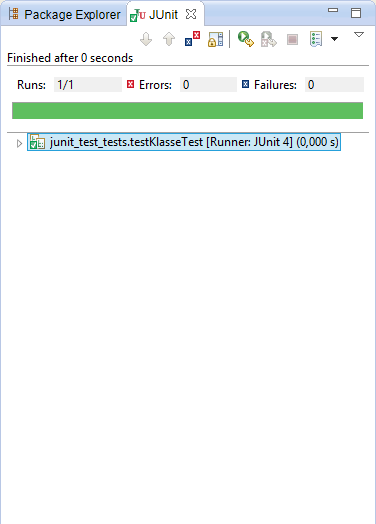
\includegraphics[width=90mm]{testsuccess.png}
\caption{Alle tests geslaagd}
\end{figure}

Voor volgende afbeelding werd een falende test toegevoegd die checkt of 1+2 gelijk is aan 12. Merk op dat onderaan meer info wordt gegeven over de gefaalde test. Er wordt duidelijk aangegeven dat de verwachte waarde 12 is, maar dat 3 de waarde is die de te testen methode returnde.

\begin{figure}[ht!]
\centering
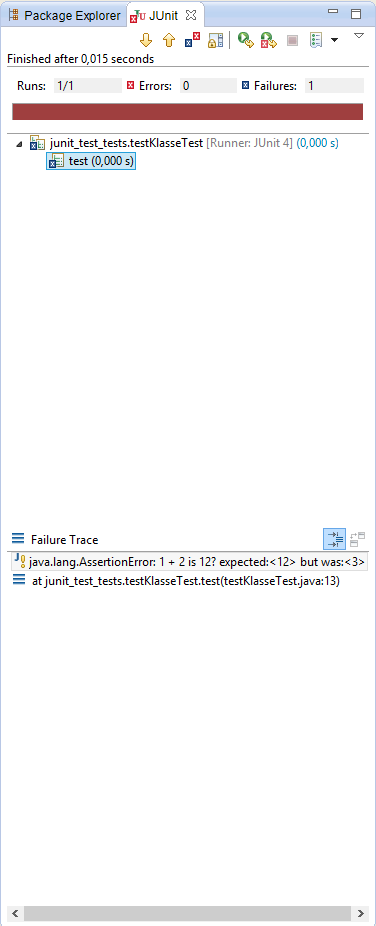
\includegraphics[width=90mm]{testfail.png}
\caption{Gefaalde test}
\end{figure}
\end{document}